\section{Résultats}

L'implémentation de base de Highcharts a été assez simple, mais la création des lignes de séparation (exemple "D'accord vs Pas d'accord") et de coche pour les réponses du salarié ont demandé plus de temps. 

Ce temps en plus est dû au temps qu'à nécessiter l'adaptation à nos besoins puisque certains n'avaient pas des fonctions par défaut pour effectuer les tâches citées ci-dessus.

\subsubsection{DWR}

DWR (Direct Web Remoting) est une librairie Java qui permet de recevoir des résultats du serveur sur le principe Ajax (asynchronous JavaScript and XML). Celui-ci permet de faire des requêtes aux serveur, de manière simplifier.

Cette librairie nous permet de faire le line entre Highcharts et notre serveur pour récupérer les informations telles que les questions et leurs valeurs (réponses et pourcentages).

\begin{figure}[H]
    \begin{center}
    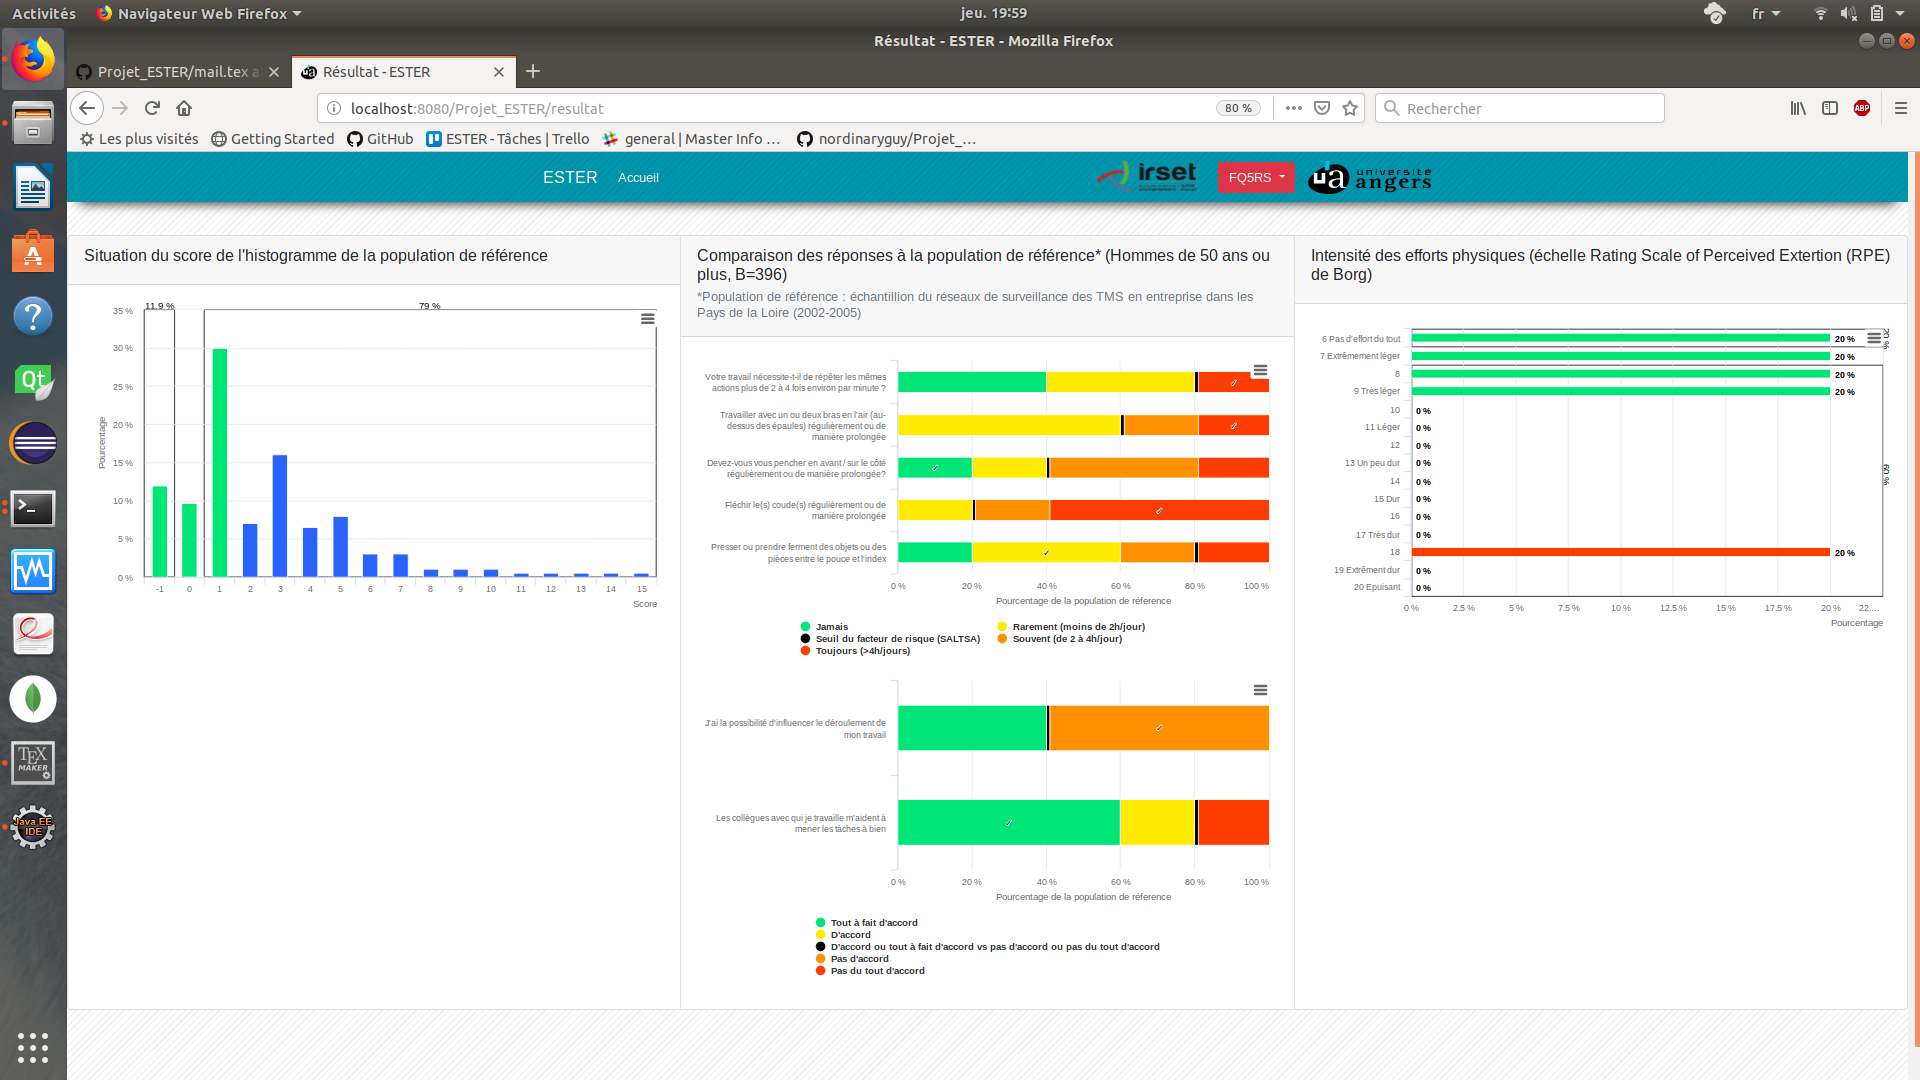
\includegraphics[scale=0.2,trim=2.8cm 0.1cm 0.8cm 5.3cm, clip=true]{img/resultat}
    \end{center}
    \caption{Mise en forme des résultats finaux rendus }
\end{figure}